\begin{figure}[h]
\centering
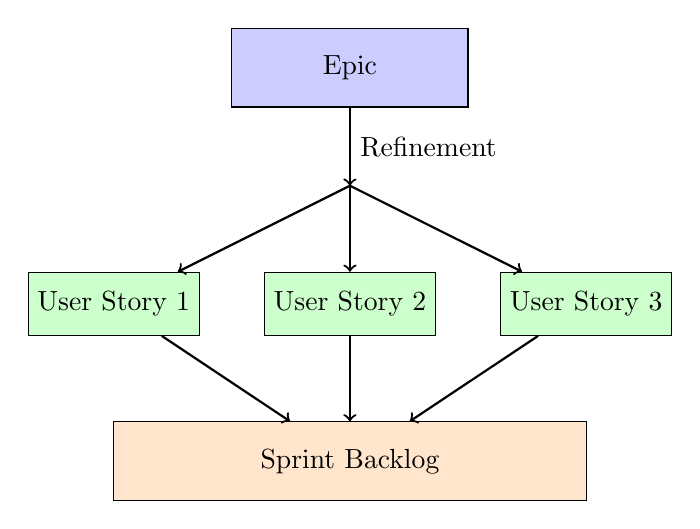
\begin{tikzpicture}
    % Epic box
    \node[draw, rectangle, fill=blue!20, minimum width=3cm, minimum height=1cm] (epic) at (0,0) {Epic};

    % Arrow down
    \draw[->, thick] (epic) -- (0,-1.5) node[midway, right] {Refinement};

    % User stories
    \node[draw, rectangle, fill=green!20, minimum width=2cm, minimum height=0.8cm] (us1) at (-3,-3) {User Story 1};
    \node[draw, rectangle, fill=green!20, minimum width=2cm, minimum height=0.8cm] (us2) at (0,-3) {User Story 2};
    \node[draw, rectangle, fill=green!20, minimum width=2cm, minimum height=0.8cm] (us3) at (3,-3) {User Story 3};

    % Arrows to user stories
    \draw[->, thick] (0,-1.5) -- (us1);
    \draw[->, thick] (0,-1.5) -- (us2);
    \draw[->, thick] (0,-1.5) -- (us3);

    % Sprint backlog
    \node[draw, rectangle, fill=orange!20, minimum width=6cm, minimum height=1cm] (backlog) at (0,-5) {Sprint Backlog};

    % Arrows to backlog
    \draw[->, thick] (us1) -- (backlog);
    \draw[->, thick] (us2) -- (backlog);
    \draw[->, thick] (us3) -- (backlog);

\end{tikzpicture}
\caption{Product Backlog Refinement Process: epics are decomposed into manageable user stories through collaborative refinement sessions.}
\label{fig:refinement-workflow}
\end{figure}
